\chapter{Using \faust Nodes}
\label{chap:run}
Once your DSP files are compiled into \ros executables, you can run them into a \ros master.

\section{Run the Master}
A \faust node needs a master to run. You can check if a master is already running by typing :
\begin{lstlisting}
rostopic list
\end{lstlisting}
Then, there are two possibilities :
\begin{itemize}
	\item either you get the following message :
	\begin{lstlisting}
ERROR: Unable to communicate with master!
	\end{lstlisting}
	which means there is no master running
	\item or you get :
	\begin{lstlisting}
/rosout
/rosout_agg
	\end{lstlisting}
	which means a master is already running.
\end{itemize}
To run a master, you have to type the following command :
\begin{lstlisting}
roscore
\end{lstlisting}

\newpage
\section{Run a \faust Node}
Now that your master is running, you can run your \faust node. It is quite simple. Type :
\begin{lstlisting}
rosrun mynodepackage mynode
\end{lstlisting}
For instance, if your node name is \textit{foo}, then type :
\begin{lstlisting}
rosrun foo foo
\end{lstlisting}
If you get an error message looking like this :
\begin{lstlisting}
[rosrun] Couldn't find executable named foo below /path/to/myworkspace/src/foo
\end{lstlisting}
then refer to section~\ref{sec:rosrun error}

\section{To Which Topics is a \faust Node Subscribing ?}
Once your \faust node is running, it automatically subscribes to topics corresponding to the parameters you can modify, and to the widgets the gtk graphic interface has. For instance, if you use a \faust node generated from the noise.dsp file (in the examples directory), the noise\_gtk node will subscribe to the topic \lstinline'noise_gtk/Volume' and the graphic interface will look like this :
\begin{figure}[ht!]
\centering
\begin{adjustbox}{minipage=5cm,margin=0pt 10pt,bgcolor=gray}
\centering
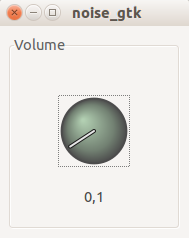
\includegraphics[scale=0.5]{images/noise_gtk.png}
\end{adjustbox}
\caption{noise\_gtk graphic interface}
\label{fig:noise_gtk}

\end{figure}
\newpage
A more complex example like the harpe.dsp file, which contains three widgets, can generate several topics to subscribe to :
\\
\begin{center}

\begin{tabular}{l}
	\lstinline'/harpe_gtk/attenuation' \\
	\lstinline'/harpe_gtk/hand' \\
	\lstinline'/harpe_gtk/level' \\
\end{tabular}\\
\end{center}
and the graphic interface can look like this :
\begin{figure}[ht!]
\centering
\begin{adjustbox}{minipage=5cm,margin=0pt 10pt,bgcolor=gray}
\centering
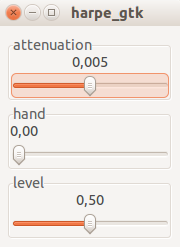
\includegraphics[scale=0.5]{images/harpe_gtk.png}
\end{adjustbox}
\caption{harpe\_gtk graphic interface}
\label{fig:harpe_gtk}
\end{figure}

If you want to change the topic name, just remap them while running your node :
\begin{lstlisting}
rosrun myfaustpackage myfaustnode /topicname:=/newtopicname
\end{lstlisting}
For instance, to remap the /harpe/hand topic to /play, then run the harpe node like this :
\begin{lstlisting}
rosrun harpe harpe /harpe/hand:=/play
\end{lstlisting}

\section{How to Escape from a Running Node ?}
To close a node running in \ros, you have two possibilities, depending on the graphic interface :
\begin{itemize}
	\item If your node has a graphic interface, then quit by clicking on the red cross in the corner of the window.
	\item If your node does not have any graphic interface, then quit by typing Ctrl+C in the node's terminal window.
\end{itemize}